\section{Modelling the problem}
\label{sec:modelling}

In this section we describe the generic mathematical model used to solve the problem.
First, the variables (see section \ref{sec:modelling:variables}) and then the 
constraints (see section \ref{sec:modelling:constraints}).

\subsection{Variables}
\label{sec:modelling:variables}

Before formulating each of the constraints, we define first the Boolean variables used:

\begin{enumerate}
    \item \label{var:box-cell} $C_{b,x,y} = 1 \Longleftrightarrow$ cell $(x,y)$ is occupied
    by box $b$. $C_{b,x,y} \in \Bool$, $\forall b,x,y$ $1 \le x \le W$, $1 \le y \le L$,
    $1 \le b \le N$.
    
    \item \label{var:box-corner} $X_{b,x,y} = 1 \Longleftrightarrow$ the top-left corner of
    box $b$ is placed at cell $(x,y)$. $X_{b,x,y} \in \Bool$, $\forall b,x,y$,
    $1 \le x \le W$, $1 \le y \le L$, $1 \le b \le N$.
    
    \item \label{var:box-rotated} $R_b \in \Bool$ indicates the rotation of box $b$. If
    $R_b = 0$ then the box is not rotated, that is, the dimensions of the box (width and
    length) are considered to be those given in the input's order: the bottom-right corner
    of box $b$ is:
    \begin{equation}
    \label{eq:box-rotation-0}
    (\Xbr, \Ybr) = (\Xtl + w_b, \Ytl + l_b)
    \end{equation}
    If $R_b = 1$ then the box is rotated, that is, the bottom-right corner of box $b$ is:
    \begin{equation}
    \label{eq:box-rotation-1}
    (\Xbr, \Ybr) = (\Xtl + l_b, \Ytl + w_b)
    \end{equation}
    (the width and length specified in the input are used in ``reverse'' order), 
    $\forall 1 \le b \le N$.
\end{enumerate}

Therefore, our model consists of two 3-dimensional matrices, each containing
$N \times W \times L$ Boolean variables, and one array of $N$ Boolean variables, giving
us a total of $N(2WL + 1)$ Boolean variables.

\subsubsection{Determining the sizes of the matrices}
\label{sec:modelling:variables:value-L}

Notice that this model has a slight drawback: using Boolean variables forces us to define
two fixed-size matrices for which we need to know the value of $L$. This is only a minor
issue since we can easily determine an upper bound on the length of the roll used: in the
worst case we might need to put all boxes ``one next to the other'' in the roll. Therefore,
in order to build the matrices we use the value
\begin{equation}
\label{eq:upper-bound-L}
L = \sum_{b=1}^N \text{max}\{w_b, l_b\}
\end{equation}

Notice that the maximum ensures a solution when the boxes are allowed to rotate: a simpler
model can be obtained by not implementing variables $R_b$ (and changing the subsequent
constraints so that boxes are not rotated at all) so that an upper bound on $L$ can be
obtained by just adding up the lengths of the input boxes, but this does not guarantee
a solution to all instances (imagine an instance where at least one box had width $w_b > W$:
without rotations this instance does not have a solution).

\subsection{Constraints}
\label{sec:modelling:constraints}

The general modelling of this problem requires 4 types of constraints
appropriate for the variable selection made.

\begin{enumerate}
    \item \label{constr:box-placed} Each box must have its top-left corner placed in the
    roll. This constraint is there to ensure that the placement contains all boxes.
    
    \begin{equation}
    \label{eq:constraint:all-boxes-used}
    \sum_{x=1}^{W} \sum_{y=1}^{L} X_{b,x,y} = 1, \qquad \forall b,\; 1 \le b \le N
    \end{equation}
    
    \item \label{constr:no-overlap} No overlapping, that is, no cell of the roll can have
    more than one box in it.
    
    \begin{equation}
    \label{eq:constraint:one-box-cell}
    \sum_{b=1}^{N} C_{b,x,y} \le 1, \qquad \forall x,y,\; 1 \le x \le W,\; 1 \le y \le L
    \end{equation}
    
    \item \label{constr:box-rot-span} Depending on the rotation of the box and its top-left
    corner's position, a box occupies certain cells of the roll. In order to speed up the
    solvers, the constraints for square boxes are simpler than those for rectangular boxes
    (because there is no need to consider a rotation for square boxes). Furthermore, since
    a box should not be placed where there is no space for it in the roll (see figure
    \ref{fig:box-out-bounds}) these constraints will not be added for these positions.
    In case it is not rotated, box $b$ cannot be placed in cell $(x,y)$ if $x + w_b > W$ or
    if $y + l_b > L$. In case it is rotated, if $x + l_b > W$ or if $y + w_b > L$.
    
    \begin{itemize}
        \item For square boxes:
        \begin{flalign}
        \label{eq:span-cells:square-boxes}
        \begin{split}
        (R_b = 0) \wedge \left( X_{b,x,y} = 1 \Longrightarrow C_{b, x + j, y + i} = 1 \right),
        & \qquad \forall b,\; 1 \le b \le N, \text{ s.t. } (w_b = l_b\; \wedge \\
        & \quad \qquad \forall x,y,\; 1 \le x \le W, 1 \le y \le L \\
        & \quad \qquad \qquad \text{ s.t. } (x + w_b \le W \wedge y + l_b \le L) \\
        & \quad \qquad \forall i,j,\; 0 \le i < l_b, 0 \le j < w_b)
        \end{split}
        \end{flalign}
        
        \item For rectangular boxes:
        \begin{flalign}
        \label{eq:span-cells:rectangular-boxes:0}
        \begin{split}
        (R_b = 0 \wedge X_{b,x,y} = 1) \Longrightarrow C_{b, x + j, y + i} = 1,
        & \qquad \forall b,\; 1 \le b \le N, \text{ s.t. } (w_b \neq l_b\; \wedge \\
        & \quad \qquad \forall x,y,\; 1 \le x \le W, 1 \le y \le L \\
        & \quad \qquad \qquad \text{ s.t. } (x + w_b \le W \wedge y + l_b \le L) \\
        & \quad \qquad \forall i,j,\; 0 \le i < l_b, 0 \le j < w_b)
        \end{split}
        \end{flalign}
        \begin{flalign}
        \label{eq:span-cells:rectangular-boxes:1}
        \begin{split}
        (R_b = 1 \wedge X_{b,x,y} = 1) \Longrightarrow C_{b, x + j, y + i} = 1,
        & \qquad \forall b,\; 1 \le b \le N, \text{ s.t. } (w_b \neq l_b\; \wedge \\
        & \quad \qquad \forall x,y,\; 1 \le x \le W, 1 \le y \le L \\
        & \quad \qquad \qquad \text{ s.t. } (x + l_b \le W \wedge y + w_b \le L) \\
        & \quad \qquad \forall i,j,\; 0 \le i < w_b, 0 \le j < l_b)
        \end{split}
        \end{flalign}
        
    \end{itemize}
    
	The constraints for the square boxes should be read as: for all boxes $b$ that are squares
	$(w_b = l_b)$, take all cells of the roll $(x,y)$ within the corresponding limits 
	$1 \le x \le W, 1 \le y \le L$ that are candidates for its top-left corner ``s.t.
	$(x + w_b \le W \wedge y + l_b \le L)$'' and, for each of these cells, impose that the
	corresponding cells occupied by $b$ according to its dimensions are occupied by it:
	$\forall i,j,\; 0 \le i < w_b, 0 \le j < l_b: X_{b,x,y} = 1 \Longrightarrow C_{b, x + j, y + i} = 1$.
	The constraints for rectangular boxes are read in a similar fashion but adding ``if the
	box is not/is rotated'' after the ``for all rectangular boxes''.

	\begin{figure}[H]
	    \centering
	    \begin{subfigure}{0.45\textwidth}
	    	\centering
			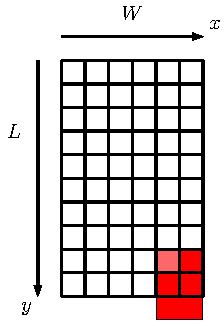
\includegraphics[scale=0.75]{out-of-bounds-no-rot.pdf}
			\centeredcaption{A non-rotated box that would be out of bounds if placed
			in the light-red cell.}
	    \end{subfigure}
	    \begin{subfigure}{0.45\textwidth}
	        \centering
	    	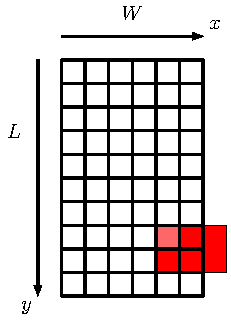
\includegraphics[scale=0.75]{out-of-bounds-rot.pdf}
	    	\centeredcaption{A rotated box that would be out of bounds if placed
	    	in the light-red cell.}
	    \end{subfigure}
	    \centeredcaption{Two situations in which a box would be out of bounds}
	    \label{fig:box-out-bounds}
	\end{figure} 
    
    \item \label{constr:box-forbid} Forbid the placement of a box in certain cells: it is
    known that, for a given rotation, a box cannot possibly be placed in certain cells of
    the roll because it would end up out of its bounds. This will stop the solvers from
    assigning positive values to these cells, that is, assign a box, in the hope that they
    detect the unfeasibility of an instance as soon as possible. Again, the constraints
    for square boxes are different from those for rectangular boxes. Moreover, it suffices
    to forbid the placement of a box's top-left corner in these cells.
    
    \begin{itemize}
        \item For square boxes:
        \begin{flalign}
        \label{eq:forbid-span-cells:square-boxes}
        \begin{split}
        X_{b,x+j,y+i} = 0,
        & \qquad \forall b,\; 1 \le b \le N, \text{ s.t. } (w_b = l_b\; \wedge \\
        & \quad \qquad \forall x,y,\; 1 \le x \le W, 1 \le y \le L \\
        & \quad \qquad \qquad \text{ s.t. } (x + w_b > W \vee y + l_b > L) \\
        & \quad \qquad \forall i,j,\; 0 \le i \le L - y, 0 \le j \le W - x)
        \end{split}
        \end{flalign}
        
        \item For rectangular boxes:
        \begin{flalign}
        \label{eq:forbid-span-cells:rectangular-boxes:0}
        \begin{split}
        R_b = 0 \Longrightarrow X_{b,x+j,y+i} = 0,
        & \qquad \forall b,\; 1 \le b \le N, \text{ s.t. } (w_b \neq l_b\; \wedge \\
        & \quad \qquad \forall x,y,\; 1 \le x \le W, 1 \le y \le L \\
        & \quad \qquad \qquad \text{ s.t. } (x + w_b > W \vee y + l_b > L) \\
        & \quad \qquad \forall i,j,\; 0 \le i \le L - y, 0 \le j \le W - x)
        \end{split}
        \end{flalign}
        \begin{flalign}
        \label{eq:forbid-span-cells:rectangular-boxes:1}
        \begin{split}
        R_b = 1 \Longrightarrow X_{b,x + j, y + i} = 0,
        & \qquad \forall b,\; 1 \le b \le N, \text{ s.t. } (w_b \neq l_b\; \wedge \\
        & \quad \qquad \forall x,y,\; 1 \le x \le W, 1 \le y \le L \\
        & \quad \qquad \qquad \text{ s.t. } (x + l_b > W \vee y + w_b > L) \\
        & \quad \qquad \forall i,j,\; 0 \le i \le W - y, 0 \le j \le L - x)
        \end{split}
        \end{flalign}
        
    \end{itemize}
    
	The constraints that forbid placing a box at a certain cell are read similarly to those
	that allow a box to be placed at a certain cell. In this case, we want those cells $(x,y)$
	that are not valid candidates for the top-left corner for a box.
    
\end{enumerate}

Notice that the modelling of these constraints may lead to a direct implementation in the
constraint programming and linear programming paradigms.
